Nowadays, many games are moving toward the gesture control system rather than 
the old joystick controls. 
Figure 1 presents an image collection of hand gestures for some English 
alphabet.

\begin{figure}[h]
\center{
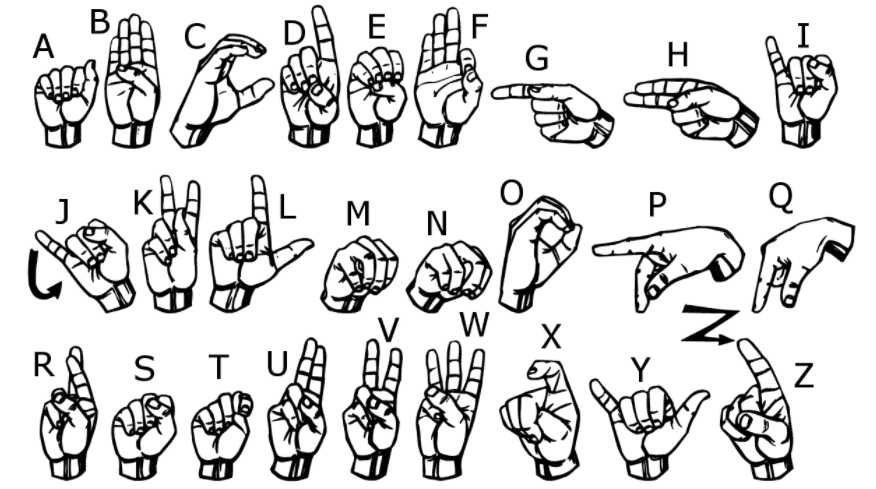
\includegraphics[width=12cm]{image/american_sign_language.png}
}
\caption{Hand Gestures for the English Alphabet}
\end{figure}

Hank wants to write a program to recognize English alphabets using sign 
language. He found that Modified National Institute of Standards and 
Technology (MNIST) database provides sing language datasets.
All samples in a dataset are byte vectors of dimension $d$. That is,
every sample can be represented by a vector $(x_1,x_2,\dots,x_d)$ where 
$x_i$ is a byte (from $0$ to $255$) for $1\le i \le d$.
Hank plans to use them to train a model and to test his program. 
He builds two sets of data. One is for training and another is for testing.

Hank is an outstanding data scientist, but his data processing skill is awful.
He accidental puts some of the training data into the testing dataset. 
This will affect the evaluation result of Hank's program.
Please write a program to help Hank to remove the training data from the 
testing dataset.
